\documentclass[11pt]{article}
\usepackage[a4paper,margin=2.5cm]{geometry}
\usepackage{graphicx}
\usepackage{hyperref}
\usepackage{booktabs}
\usepackage{amsmath}
\usepackage[T1]{fontenc}

\title{GB reweighting of MC to data on reconstructed direction\\
\large Documentation of the pipeline and the first ROC sanity check}
\author{Holger}
\date{}

\begin{document}
\maketitle

\section*{Purpose}

This note documents the pipeline that produces the plot
roc\_mc\_vs\_data\_before\_after.png and the two weight files
GB\_and\_base\_weights\_stopped.csv and
GB\_and\_base\_weights\_through.csv. The goal is to reweight the
Monte Carlo (MC) muon sample so that its reconstructed
\textit{(zenith, azimuth)} distribution matches that of data, separately for
events classified as stopped and through\nobreakdash-going. All other
reconstructed observables (energy, $z$\nobreakdash-position, track length,
charge, $N_{\text{hits}}$, \dots) are deliberately kept as
\emph{unreweighted} variables, so that they can later be used as blind
validation tests of how well MC reproduces data.

\section{Inputs}

\paragraph{MC sample.}
File:
\begin{center}
MC\_vs\_BS\_analysis/MC/muons\_1305k\_130000\_720k\_139008.db
\end{center}
Contains $\sim 2.0$\,M simulated muon events with standard pulse maps
(SplitInIcePulses) and a truth table with the physics weight
norm\_class\_this\_db\_osc\_weight (oscillation/flux weighting,
used as the MC \emph{base weight} throughout).

\paragraph{Data sample.}
File:
\begin{center}
MC\_vs\_BS\_analysis/Data/data\_IC86.21\_withrates.db
\end{center}
Real IceCube data from IC86 with $\sim 4$\,M events and the per\nobreakdash-event
rate weight subrun\_weight (used as the data \emph{base weight}).
The data sample is pre\nobreakdash-filtered by a muon PID score: we retain only
events with
\begin{center}
pid\_muon\_logit\_data $=\operatorname{logit}\bigl(\text{pid\_muon\_pred}\bigr) > 5$,
\end{center}
where pid\_muon\_pred is stored in
\begin{center}
data\_IC86\_2021\_with\_subrun\_PID\_888826.csv
\end{center}
and logit is computed with a small $\varepsilon$-stabilisation to avoid
$\log(0)$. This leaves $\sim 1.9$\,M high\nobreakdash-purity data muons.

\section{Reconstructions applied}

Two transformer models were run in inference mode on \emph{both} the MC and
the data sample, with identical pipelines so that MC and data are compared
apples to apples.

\paragraph{Stopped / through\nobreakdash-going classifier.}
Model:
\begin{center}
ThroughOrStopped\_muon/results/stopped\_transformer\_2M/best\_model.pt
\end{center}
This is a pulse\nobreakdash-level transformer that outputs a single logit per
event. We apply a $\sigma$ and keep the score. Outputs are written to
\begin{center}
ThroughOrStopped\_muon/inference/output/stopped\_recon\_*.csv
\end{center}
with columns event\_no, stopped\_logit, stopped\_score, stopped\_pred.

\paragraph{Zenith / azimuth regressor.}
Model: Inar's direction transformer,
\begin{center}
Classifiers/Inars\_zenith\_azimuth\_transformer\_recon/results/transformer\_720k\_muons/best\_model.pt
\end{center}
The training configuration uses position\nobreakdash-mode pulse grouping on the
feature set [dom\_x, dom\_y, dom\_z, dom\_time, charge, width], so the inference
script forces the \emph{same} feature set for both MC and data (instead of
letting the auto\nobreakdash-detect pick sensor\_id mode on the data DB,
which would have used a different collator). Outputs are written to
\begin{center}
MC\_vs\_BS\_analysis/zenith\_azimuth\_inference/output/zenaz\_recon\_*.csv
\end{center}
with columns event\_no, zenith\_pred, azimuth\_pred.

\section{GB reweighting procedure}

The reweighting is implemented in
\begin{center}
MC\_vs\_BS\_analysis/GBreweighting/fit\_GBreweighter.py
\end{center}

\begin{enumerate}
    \item Merge stopped\_recon, zenaz\_recon and base
          weights from the truth table on event\_no for each of
          MC and data.
    \item Split each sample at stopped\_score $> 0.5$, producing
          four populations: $\text{MC}_{\text{stopped}}$,
          $\text{MC}_{\text{through}}$, $\text{data}_{\text{stopped}}$,
          $\text{data}_{\text{through}}$.
    \item For each class, fit a hep\_ml.reweight.GBReweighter on
          the 2D feature space (zenith\_pred, azimuth\_pred),
          mapping MC\,$\to$\,data. The fit uses
          original\_weight = base\_weight$_\text{MC}$ and
          target\_weight = base\_weight$_\text{data}$, so the
          target distribution is the \emph{physically weighted} data
          distribution, not the raw event count.
    \item To avoid overfitting while keeping every event, a 2\nobreakdash-fold
          cross\nobreakdash-reweighting scheme is used: MC and data are each split
          50/50 (fold A, fold B). Two GBReweighters are fitted, one on
          MC$_A \to$ data$_A$ and one on MC$_B \to$ data$_B$. Each MC event
          then receives a gb\_weight from the reweighter that did
          \emph{not} see it. Data events get
          gb\_weight $\equiv 1$.
    \item gb\_weight is then globally rescaled so that
          $\sum \mathrm{base\_weight}_{\mathrm{MC}} \cdot \mathrm{gb\_weight}$
          matches $\sum \mathrm{base\_weight}_{\mathrm{data}}$ within the
          class, so that the rate normalisation is carried by the base
          weights and the GB factor only fixes the shape.
    \item The final per\nobreakdash-event weight is
          final\_weight = base\_weight $\cdot$ gb\_weight.
\end{enumerate}

The output is two CSV files (one per class) with columns
event\_no, source (mc/data),
base\_weight, gb\_weight, final\_weight.

\paragraph{GBReweighter hyperparameters.}
n\_estimators=80, learning\_rate=0.1,
max\_depth=3, min\_samples\_leaf=200,
subsample=0.6.

\section{Sanity check: MC\,vs\,data classifier ROC}

As a closure test, a scikit\nobreakdash-learn
GradientBoostingClassifier (50 trees, depth 3) is trained to
distinguish MC from data on the same 2D feature space
(zenith\_pred, azimuth\_pred), once using
base\_weight and once using final\_weight. A 50/50 train/test
split is used and both AUC and ROC are computed with
sample\_weight. The result is saved to
\begin{center}
plots/roc\_mc\_vs\_data\_before\_after.png
\end{center}

\begin{figure}[h]
    \centering
    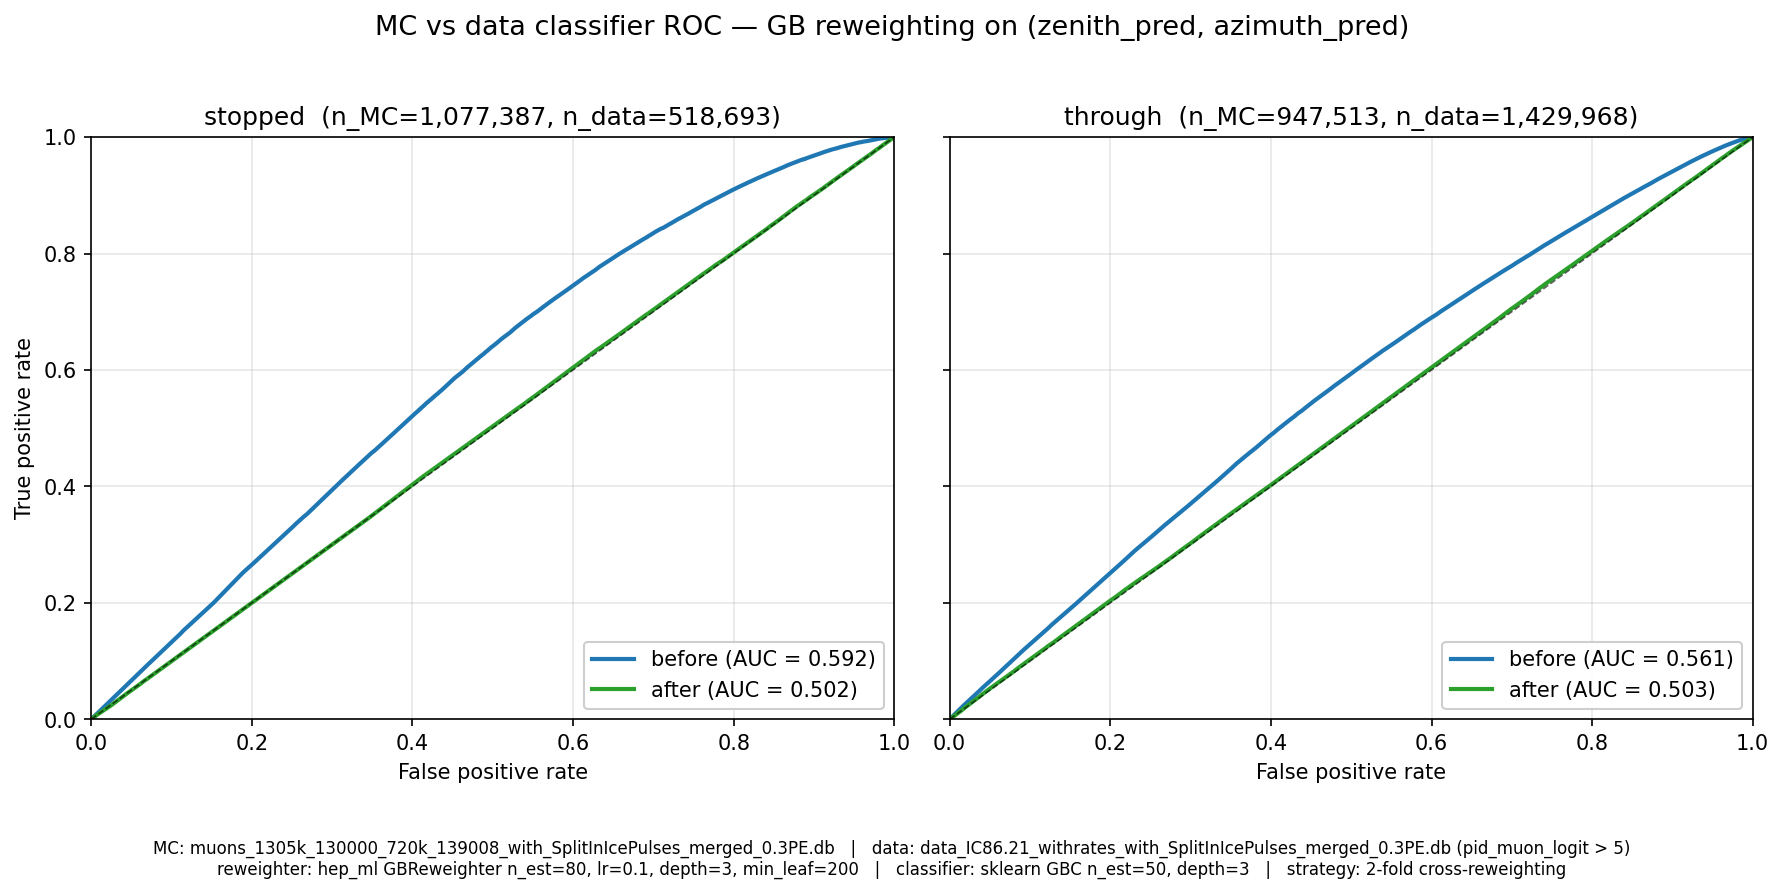
\includegraphics[width=\linewidth]{../plots/roc_mc_vs_data_before_after.png}
    \caption{MC vs data classifier ROC, one subplot per class (stopped and
    through), showing the curve before (blue) and after (green) GB
    reweighting on (zenith\_pred, azimuth\_pred).
    The dashed diagonal is random ($\text{AUC}=0.5$). Event counts
    $n_{\text{MC}}$ and $n_{\text{data}}$ per class are shown in the
    subplot titles, and the footer lists the data and MC sources as well
    as the reweighter/classifier hyperparameters.}
    \label{fig:roc_before_after}
\end{figure}

\subsection*{Interpretation}

The \emph{before} AUC is small (around $0.55$) for both classes. This is
\textbf{not} a sign that the sanity\nobreakdash-check classifier is weak --- it is
the physical statement that the 2D marginal of
(zenith\_pred, azimuth\_pred) is already quite similar
between (weighted) MC and (weighted) data. A two\nobreakdash-feature BDT
essentially has nowhere to go. After the cross\nobreakdash-reweighting the AUC
drops further towards the random baseline $0.5$, confirming that the
reweighter closes the small residual gap in the same 2D space it was
fitted on.

A direct comparison with a full\nobreakdash-pulse DynEdge MC\,vs\,BS classifier
\begin{center}
scripts/separate\_mc\_bs\_with\_dynedge.py
\end{center}
would produce a much
higher AUC, but that number measures something different: it quantifies
how distinguishable MC and data are on the \emph{full pulse image}, i.e.\
also through all the variables we deliberately did \emph{not} reweight on
(energy, position, charge, hit topology, \dots). Those variables are the
next step in the analysis: they act as blind tests of how faithfully MC
reproduces data, now that direction has been reweighted away.

\section{Status and next step}

\paragraph{Done.}
\begin{itemize}
    \item Stopped/through recon for MC and for PID\nobreakdash-filtered data.
    \item Zenith/azimuth recon for MC and for PID\nobreakdash-filtered data,
          using Inar's direction transformer with a forced
          position\nobreakdash-mode pipeline to be identical on both samples.
    \item Class split at stopped\_score $>0.5$.
    \item 2\nobreakdash-fold cross GB reweighting on
          (zenith\_pred, azimuth\_pred) per class,
          with MC base weight norm\_class\_this\_db\_osc\_weight
          and data base weight subrun\_weight.
    \item ROC closure check before/after reweighting, one subplot per
          class.
\end{itemize}

\paragraph{Next.}
A plot script that compares MC and data on the test variables
(energy\_pred, position\_z\_pred, track length, $Q_\text{tot}$,
$N_\text{hits}$, $t_\text{std}$, DOM $x,y,z$, rde, pmt\_area,
saturation fraction, HLC/SLC charge) using final\_weight, and a
second BDT trained on those variables to quantify the remaining
MC/data discrepancy outside the reweighted directional subspace.

\end{document}
